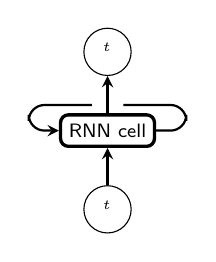
\begin{tikzpicture}[x=1cm, y=1cm, >=stealth, font=\sffamily\scriptsize]
    \tikzstyle{neuron}=[circle, draw, minimum size=.6cm]
    \tikzstyle{Arrow}=[rounded corners=.20cm,thick] % Arrows with rounded corners
    \tikzstyle{cell}=[% For the main box
        rectangle,
        draw,
        rounded corners=1mm,
        very thick,
        minimum width=6mm,
        minimum height=4mm,
        inner sep=3pt
        ]
    % Input node
    \node [neuron] (input) at (0,0) {$\x^\vbra{t}$};
    
    % Recurrent cell
    \node [cell] (cell) at (0,1) {RNN cell};
    
    % Output node
    \node [neuron] (output) at (0,2) {$\h^\vbra{t}$};
    
    % Feedforward arrows
    \draw [->, Arrow] (input) -- (cell);
    \draw [->, Arrow] (cell) -- (output);
    
    % Feedback arrows
    \draw [-, Arrow] (cell.east) -- (1, 1) -- (1, 1.325) -- (0.2, 1.325);
    \draw [<-, Arrow] (cell.west) -- (-1, 1) -- (-1, 1.325) -- (-0.2, 1.325);
\end{tikzpicture}